\documentclass[12pt,letterpaper]{article}
\usepackage{preamble}

%%%%%%%%%%%%%%%%%%%%%%%%%%%%%%%%%%%%%%%%%%
%%%% Edit These for yourself
%%%%%%%%%%%%%%%%%%%%%%%%%%%%%%%%%%%%%%%%%%
\newcommand\course{MIE231}
\newcommand\hwnumber{1}
\newcommand\userID{Andrew Zhang 1004996533}
\renewcommand{\arraystretch}{2}

\begin{document}
    \begin{figure}[H]
        \centering
        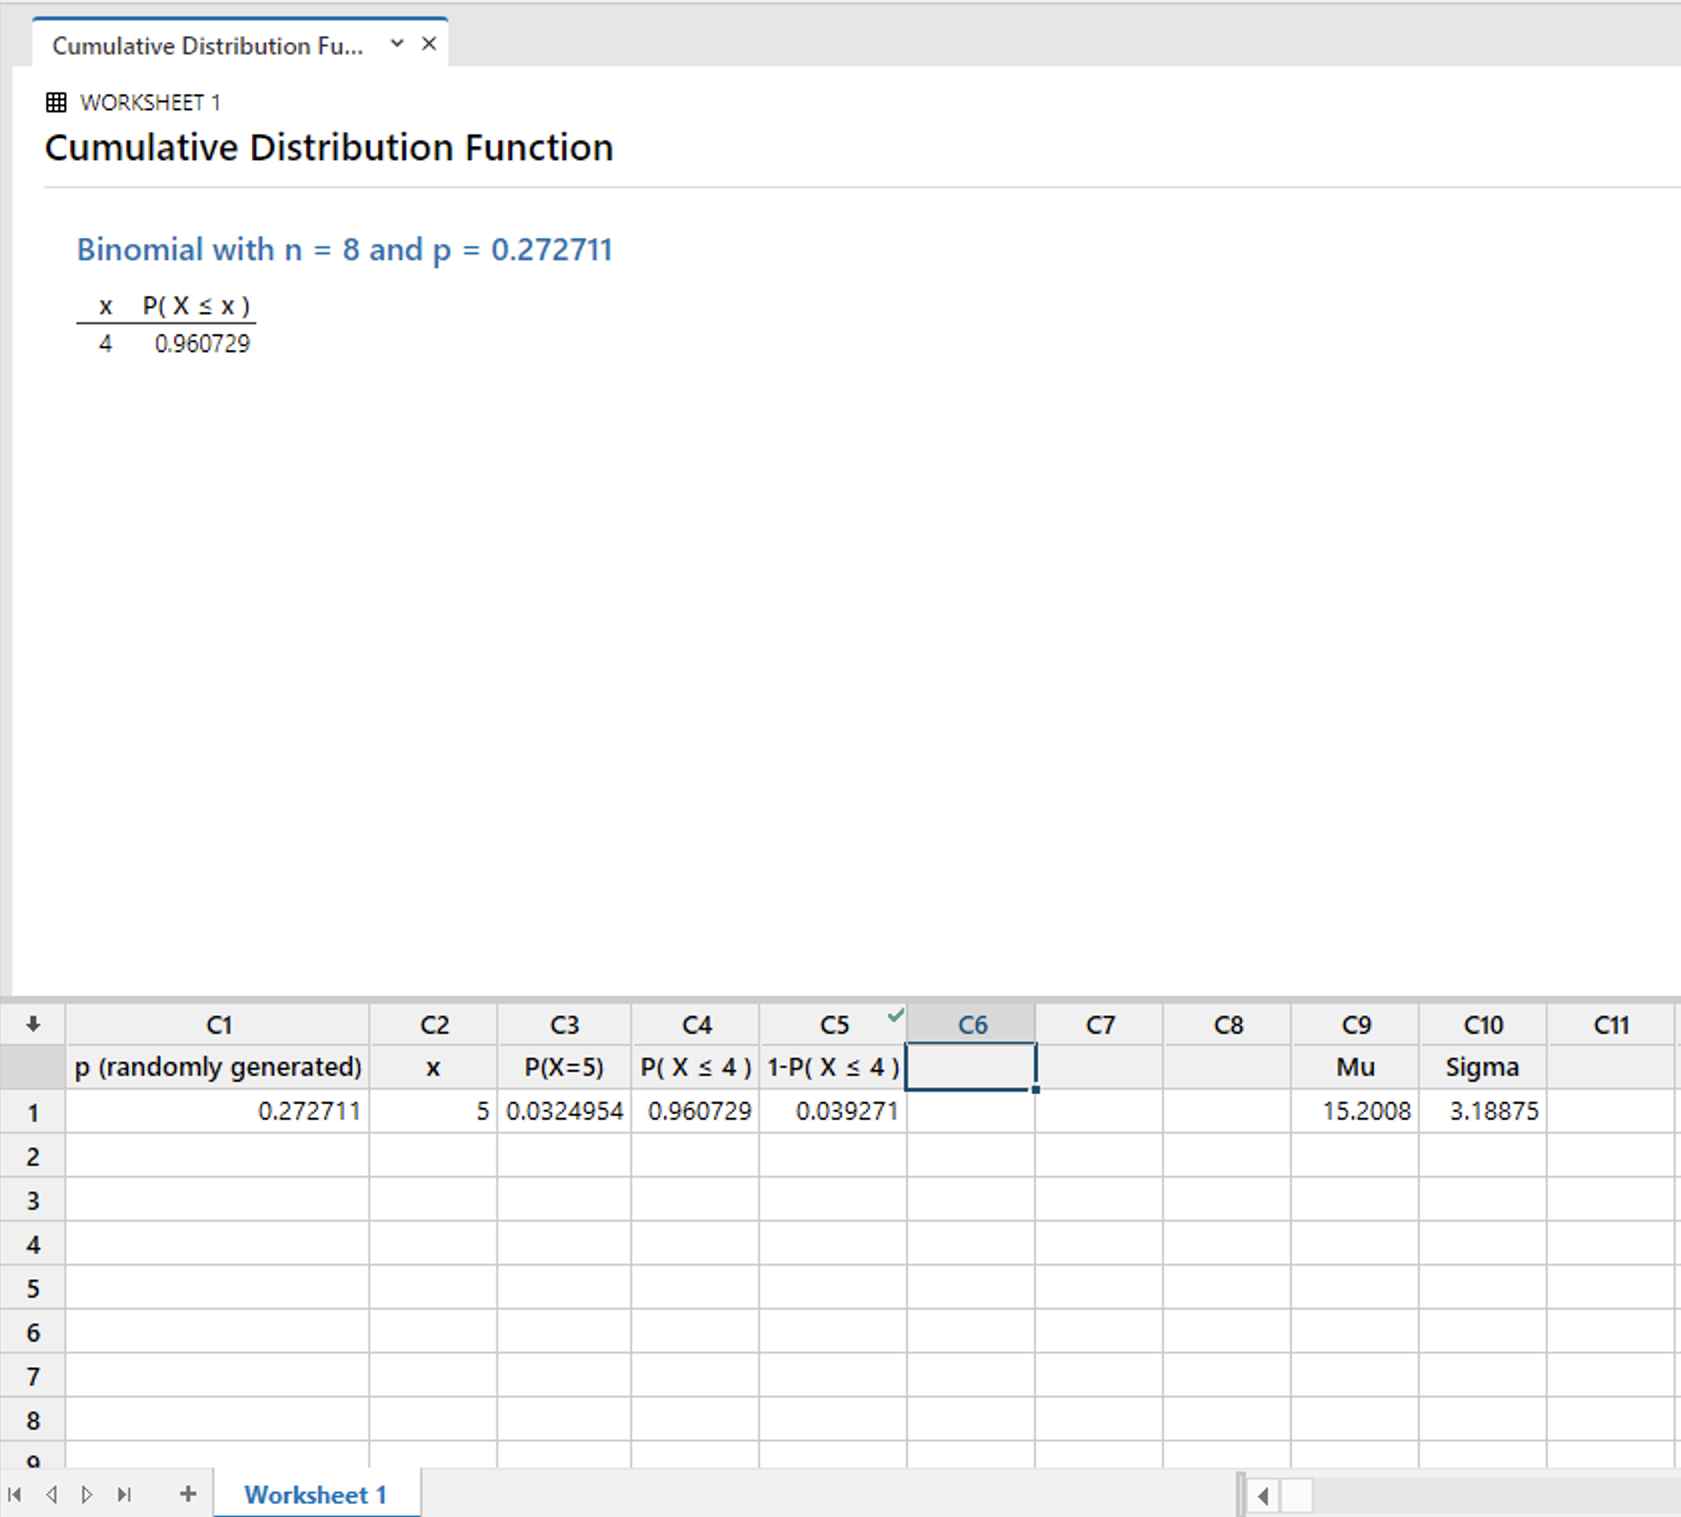
\includegraphics[width = 16cm]{images/fullWorkv2.png}
        \caption{Minitab Worksheet}
    \end{figure}

\begin{enumerate}[leftmargin=!,labelindent=5pt]
    \item  From C1 in Figure 1, $p = 0.272711$. This is the proportion of the binomial distribution.

        
    \item P$(X = x)$ is calculated in C3 using the value for $x$ in C2.
    
    \begin{center}
    P$(X= 5)$ = 0.0324954
    \end{center}
        
    \item From C4, P$(X \leq 4)$ = 0.960729. P$(X \geq 5)$ is then calculated in C5 as follows
    \begin{center}
    P$(X \geq 5)$ $= 1-$P$(X \leq 4)$ $= 0.039271$
    \end{center}
        \newpage
    \item  From C9 and C10, $\mu= 15.2008,\quad \sigma_x = 3.18875$.
    \item $(1-\alpha) = 0.99 \Rightarrow \frac{\alpha}{2} = 0.005$.
        From z distribution table,
        $$z_{\frac{\alpha}{2}} = -2.575,\quad z_{(1-\frac{\alpha}{2})} = 2.575$$
        
        Formula for sample means: 
        \begin {align}
            \nonumber
             z &= \frac{\bar{x} - \mu}{\frac{\sigma_{x}}{\sqrt{n}}}\\
            \nonumber\\
            \Rightarrow \:\bar{x}  &= (z)\left(\frac{\sigma_x}{\sqrt{n}}\right)+ \mu
            \nonumber
        \end {align}
        $$
        \begin{tabular}{|c|c|c|}
            \hline
            \textbf{n}: & \textbf{Lower limit of $\bar{x}$} &\textbf{Upper limit of $\bar{x}$}\\
            & $z = z_{\frac{\alpha}{2}}$ &$z = z_{(1-\frac{\alpha}{2})}$\\\hline \hline
            4 & $\bar{x}_l = (-2.575)\left(\frac{3.18875}{\sqrt{4}}\right)+ 15.2008$ & $\bar{x}_u = (2.575)\left(\frac{3.18875}{\sqrt{4}}\right)+ 15.2008$ \\
            & $\bar{x}_l = 11.095$ & $\bar{x}_u = 19.306$\\\hline
            16 & $\bar{x}_l = 13.148$  & $\bar{x}_u = 17.254$ \\\hline
            64 & $\bar{x}_l= 14.174$ & $\bar{x}_u = 16.227$ \\\hline
            256 & $\bar{x}_l =14.687$ & $\bar{x}_u=15.714$ \\ \hline

        \end{tabular}
        $$
    
\end{enumerate}
\end{document}
